\chapter{Caso de estudio}
\label{capitulo6}
Para mostrar el uso de la herramienta se simulo en un ambiente virtualizado la interacción y colaboración entre varios CSIRTs. Mediante esta prueba se realizó el intercambio de cyber observables entre las distintas organizaciones. Dicho intercambio se realizo utilizando los distintos servicios provistos por TAXII.

\section{Objetivos}

El caso de estudio fue ideado con la finalidad de validar la implementación del protocolo TAXII realizada así como las distintas interacciones entre RTIR y la aplicación TAXII. 

Para realizar la validación de las interacciones entre RTIR y la aplicación TAXII se tuvó como objetivo recorrer cada una de las interfaces implementadas.

La validación del protocolo TAXII se realizó mediante la invocación de cada una de las funcionalidades que implementan el intercambio de información. Dicha invocación se realizó desde la interfaz de RTIR mediante la API REST implementada durante el proyecto. El protocolo implementado se validó de dos maneras, primero mediante dos instancias de la aplicación TAXII implementada y luego por medio de YETI. Como se dijó anteriormente YETI es una implementación de referencia del protocolo TAXII provista por MITRE.

\section{Escenario del caso de estudio}
Se utilizaron dos máquinas vistuales para realizar la prueba de concepto, cada una de ellas tiene instalada Linux Mint 17. En dichos equipos se instaló RTIR junto con TAXIIApp. Además en la máquina virtual correspondiente al CSIRT2 se instalo YETI. Cada una de estas máquinas virtuales tiene incluida una base de datos con esquemas correspondientes a cada una de las aplicaciones. En la figura \ref{fig.laboratorio_desplegado} se ve un esquema representando el despliegue realizado.

\begin{figure}[h!]
	\label{fig.laboratorio_desplegado}
	\centering
	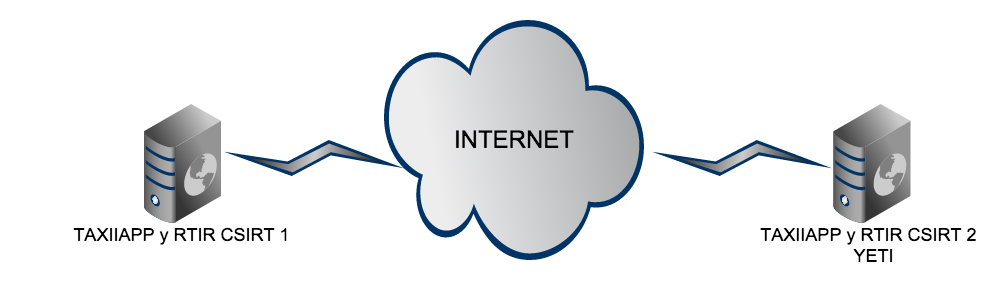
\includegraphics[scale=0.4]{caso-de-estudio/laboratorioDesplegado.png}
	\caption{Despliegue realizado para el caso de estudio}
\end{figure}

La tabla que se presenta a continuación indica la información respecto al laboratorio implementado.
\renewcommand{\tablename}{Tabla}

\begin{table}
	\begin{center}
		\begin{tabular}{|c|c|c|c|c|}
			\hline
			Equipo & Hostname & Ip & Puerto & Aplicación \\ \hline
			CSIRT 1 & csirt1.com & 172.16.59.219 & 8080 & RTIR \\ \hline
			CSIRT 1 & csirt1.com & 172.16.59.219 & 8001 & TAXIIApp \\ \hline
			CSIRT 2 & csirt2.com & 172.16.59.218 & 8080 & RTIR \\ \hline
			CSIRT 2 & csirt2.com & 172.16.59.218 & 8001 & TAXIIApp \\ \hline
			CSIRT 2 & csirt2.com & 172.16.59.218 & 9080 & YETI \\ \hline
		\end{tabular}
	\end{center}
	\caption{Información de cada equipo}
	\label{tabla_equipos}
\end{table}

En la tabla \ref{tabla_equipos} se muestran las direcciones ip para cada uno de los equipos utilizados en el caso de estudio. En el CSIRT 1 se tiene instalado RTIR con el \textit{plugin} implementado durante el proyecto para comunicarse con TAXIIApp. También se tiene instalado TAXIIApp para realizar los intercambios de información con el protocolo TAXII. RTIR escucha en el puerto 8080 mientras que TAXIIApp en el 8001.
Dichas aplicaciones se encuentras instaladas también en el CSIRT 2 escuchando en los mismos puertos. A su vez en el CSIRT 2 se encuentra una instalación de YETI. Dicha instalación se encuentra escuchando en el puerto 8080. YETI y TAXIIApp se encuentran corriendo ambas en el mismo equipo para no tener una maquina virtual extra.
En cada uno de los equipos se encuentra instalada una base de datos Mysql en la que se encuentran los esquemas de base de datos utilizados por cada una de las aplicaciones.

\section{Ejecución del caso de estudio}
La figura \ref{fig.flujos} siguiente muestra cuales fueron los pasos para realizar el intercambio entre las distintas organizaciones.

\begin{figure}[H]
	\centering
	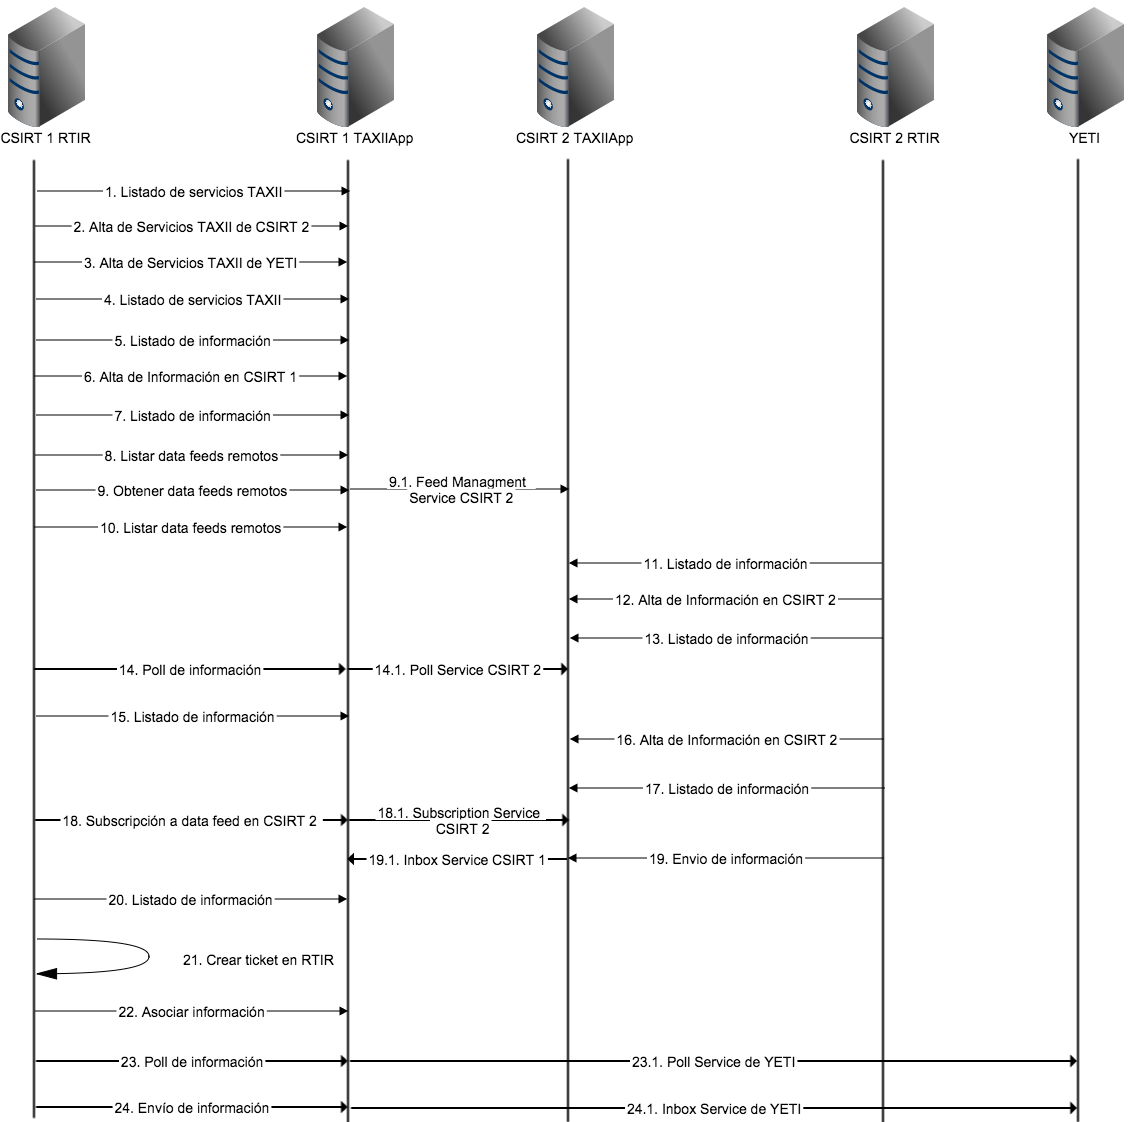
\includegraphics[scale=0.35]{caso-de-estudio/flujos.png}
	\caption{Flujos realizados por el caso de estudio}
	\label{fig.flujos}
\end{figure}

En los pasos 1 a 4 de la figura \ref{fig.flujos} agregamos en el CSIRT 1 los servicios TAXII correspondientes a TAXII App y a YETI, ambos ejecutándose en el CSIRT 2.
En el caso de TAXII App se agregaron todos los servicios necesarios para realizar el intercambio. Sin embargo, la implementación de YETI solo cuenta con el \textit{inbox service}, \textit{poll service} y \textit{discovery service}, por lo tanto se agregaron \textit{inbox service} y \textit{poll service} como los servicios en YETI. La implementación de TAXII realizada durante el proyecto no implementó el \textit{discovery service} y por ello fue necesario implementar un caso de uso para ingresar los servicios. \\
\bigskip
En la figura \ref{fig.regservicios} observamos el ingreso de los servicios TAXII y en la figura \ref{fig.lstservicios} el listado de los servicios ingresados anteriormente.

\begin{figure}[H]
	\centering
	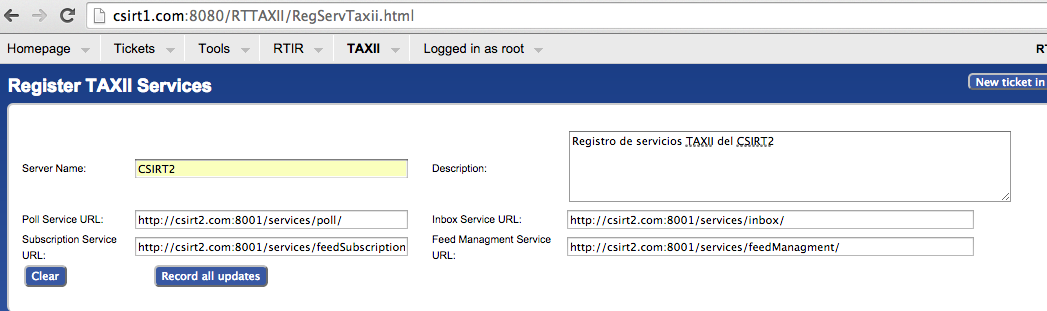
\includegraphics[scale=0.4]{caso-de-estudio/RegistroServicios.png}
	\caption{Registro de Servicios TAXII}
	\label{fig.regservicios}
\end{figure}

\begin{figure}[H]
	\centering
	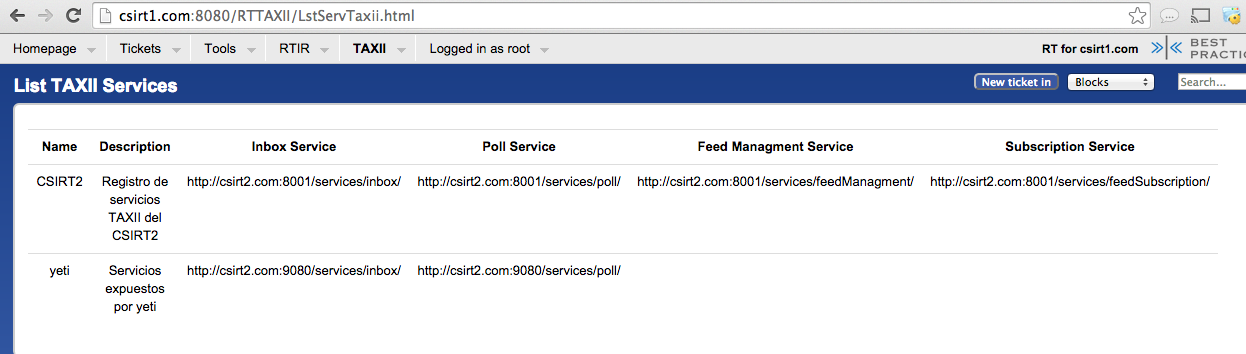
\includegraphics[scale=0.35]{caso-de-estudio/listadoservicios.png}
	\caption{Listado de Servicios TAXII}
	\label{fig.lstservicios}
\end{figure}

En los pasos 5 a 7 de la figura \ref{fig.flujos} se ingresa nueva información en el CSIRT 1, a su vez se comprueba que la información se halla dado de alta adecuadamente en el sistema. Lo mismo se realiza en los pasos 11 a 13, 16 y 17, la diferencia que esta vez se realiza desde el CSIRT 2, dicha información será luego enviada al CSIRT 1 por medio del poll service así como del inbox service.
En la figura \ref{fig.altacorreo} se ve el ingreso de información, se da de alta un Cyber observable que representa un correo electrónico que podría provenir por ejemplo de un ataque de phishing. En el anexo se pueden ver los distintos cyber observables dados de alta, los cuales se obtuvieron de MITRE(\cite{mitre}).

En la figura \ref{fig.lstinfo} se observa información dada de alta en el sistema, también se ve información que fue obtenida por medio del poll service del data feed “default” del CSIRT 2.

\begin{figure}[H]
	\centering
	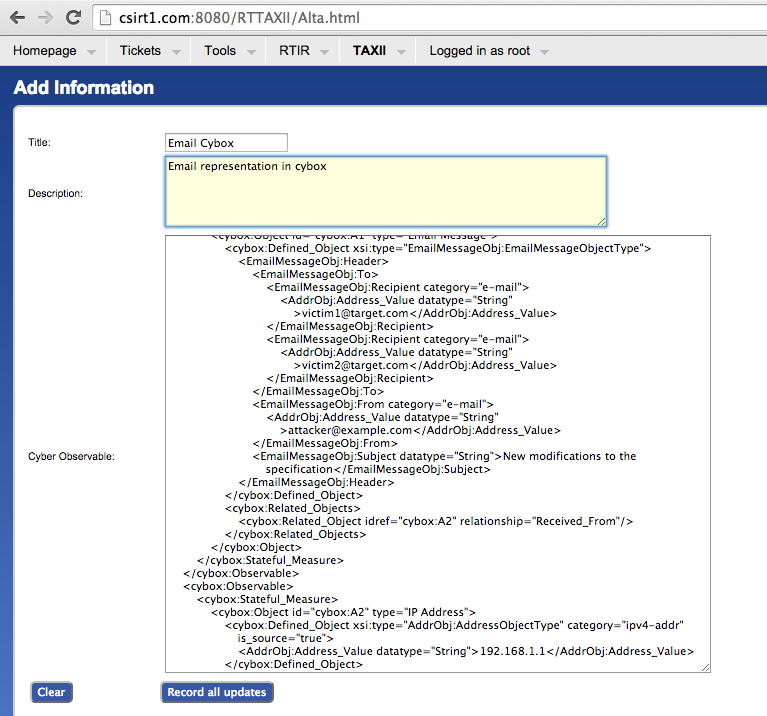
\includegraphics[scale=0.6]{caso-de-estudio/alta.png}
	\caption{Alta de información de correo electrónico}
	\label{fig.altacorreo}
\end{figure}

\begin{figure}[H]
	\centering
	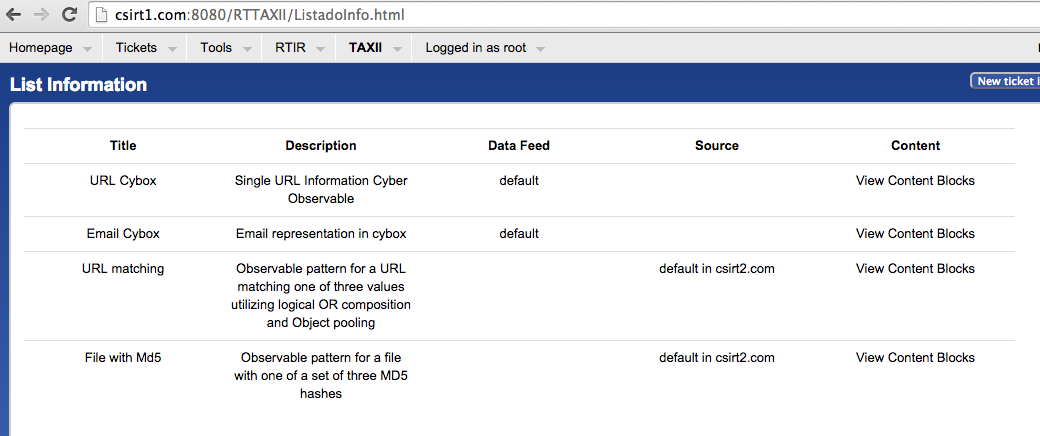
\includegraphics[scale=0.3]{caso-de-estudio/listadoInfo.png}
	\caption{Listado de información en el sistema}
	\label{fig.lstinfo}
\end{figure}

Los pasos 8 a 10 se encargan de la obtención de los data feeds en el CSIRT 2 y a su vez se comprueba que los data feeds se hayan obtenido correctamente. Para obtener los data feeds se envía un mensaje desde TAXII App en el CSIRT 1 solicitándolos al CSIRT 2. \\
La figura \ref{fig.obtremote} muestra la obtención de los data feeds remotos en el CSIRT 2, luego en la figura \ref{fig.lstremotedf} se ve un listado del data feed obtenido. A su vez se ve el data feed de YETI.

\begin{figure}[H]
	\centering
	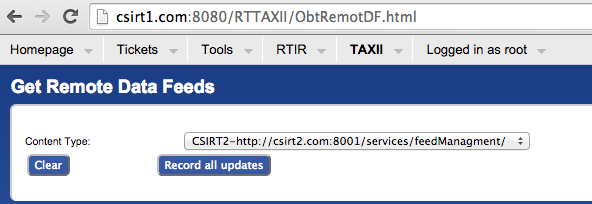
\includegraphics[scale=0.5]{caso-de-estudio/obtremote.png}
	\caption{Obtención de data feeds remotos}
	\label{fig.obtremote}
\end{figure}

\begin{figure}[H]
	\centering
	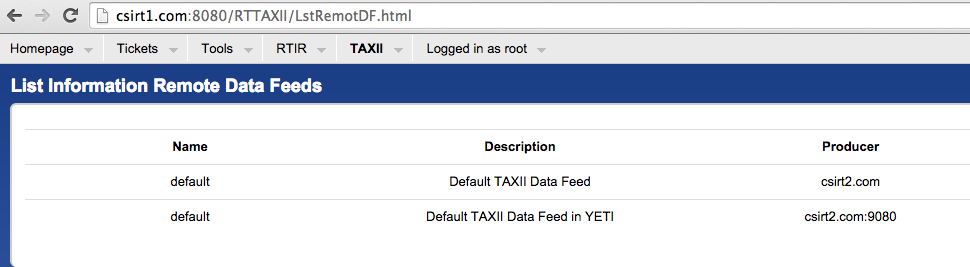
\includegraphics[scale=0.4]{caso-de-estudio/lstremotedf.png}
	\caption{Data feeds en otras organizaciones}
	\label{fig.lstremotedf}
\end{figure}

En el paso 14 se realiza el poll de información, para ello se invoca al poll service en el CSIRT 2, esto devuelve toda la información en el data feed especificado. Luego de realizado este paso, se lista nuevamente la información para ver cuales fueron los datos recibidos.
En la figura \ref{fig.pollinfo} se ve el polling de información. Previamente se vio el listado de información luego de hacer el poll.

\begin{figure}[H]
	\centering
	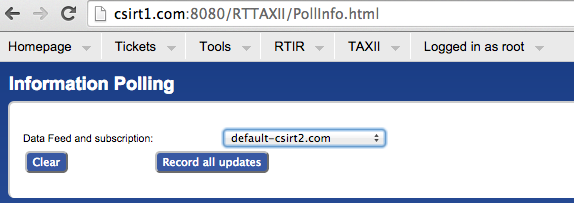
\includegraphics[scale=0.4]{caso-de-estudio/pollinformacion.png}
	\caption{Poll de información}
	\label{fig.pollinfo}
\end{figure}

Como se dijo anteriormente, en los pasos 16 y 17 se ingresa nueva información al CSIRT 2, dicha información es agregada para luego ser enviada al inbox del CSIRT 1. Previo a ser enviada, el CSIRT 1 debe registrarse para indicar que desea recibir información al inbox service. Dicha subscripción se realiza en el paso 18 invocando al servicio de feed managment del CSIRT 2. Luego de esto, en el paso 19, se envía la información al inbox service del CSIRT 1 desde el CSIRT 2.
En el paso 20 se observan los nuevos datos obtenidos luego de que se envíe la información al inbox service del CSIRT 1.

En las figuras \ref{fig.subfeed} y \ref{fig.subdf} se ve la subscripción a un data feed en otra organización, mientras que en la \ref{fig.relacInfo} se ve el envío de información que se realizará por medio de inbox service como se dijo anteriormente.

\begin{figure}[H]
	\centering
	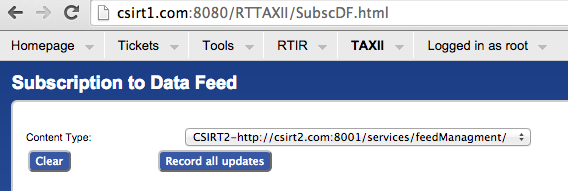
\includegraphics[scale=0.4]{caso-de-estudio/subscriptionfeed.png}
	\caption{Primer paso de subscripción a data feeds}
	\label{fig.subfeed}
\end{figure}

\begin{figure}[H]
	\centering
	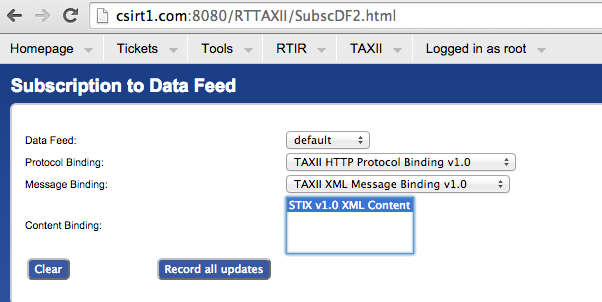
\includegraphics[scale=0.4]{caso-de-estudio/subscriptiondf.png}
	\caption{Segundo paso de subscripción a data feeds}
	\label{fig.subdf}
\end{figure}

\begin{figure}[H]
	\centering
	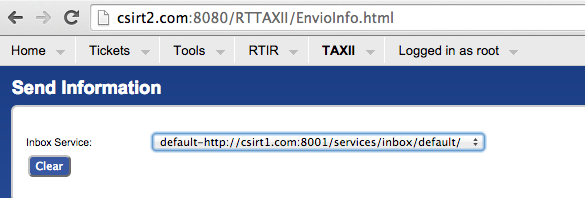
\includegraphics[scale=0.4]{caso-de-estudio/envioInfo.png}
	\caption{Envio de información}
	\label{fig.envioInfo}
\end{figure}

En el paso \ref{fig.envioInfo} se crea un nuevo ticket en el RTIR, dicho ticket será asociado con información existente en TAXII App. Dicha información puede haber sido obtenida de uno de los otros CSIRTs o de ingresada por un analista localmente.

En la figura \ref{fig.lstRelacInfo} se ve la asociación entre tickets del RTIR e información almacenada en TAXIIApp.

\begin{figure}[H]
	\centering
	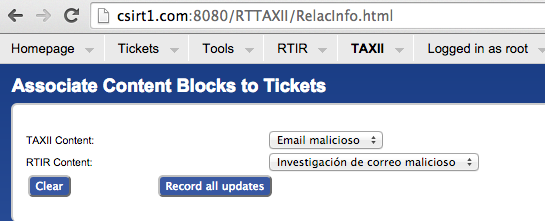
\includegraphics[scale=0.4]{caso-de-estudio/relacInfo.png}
	\caption{Asociación entre Tickets y Content blocks}
	\label{fig.relacInfo}
\end{figure}

\begin{figure}[H]
	\centering
	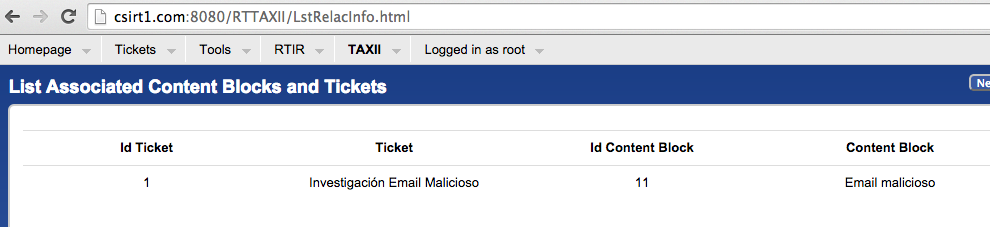
\includegraphics[scale=0.4]{caso-de-estudio/lstRelacInfo.png}
	\caption{Listado de asociaciones existentes}
	\label{fig.lstRelacInfo}
\end{figure}

Finalmente se invoca al poll service de YETI para obtener información y luego se envía información a YETI utilizando su inbox service. Como se dijo anteriormente, YETI no tiene todos los servicios implementados y además no puede iniciar el intercambio de información. Como YETI  no implementa el manejo de subscripciones u obtenciones de data feeds, se ingreso previamente dicha información de YETI en el CSIRT 1.